\documentclass{standalone}

\usepackage{tikz}
\usepackage{circuitikz}

\tikzset{block/.style = {draw, fill=white, very thick, rectangle, minimum height=1cm, minimum width=2cm},
         lblock/.style={draw,fill=white,very thick, rectangle, minimum height=3cm, minimum width=1cm},
         sum/.style= {draw, fill=white, very thick, circle, node distance=0.5cm}}

         
\begin{document}
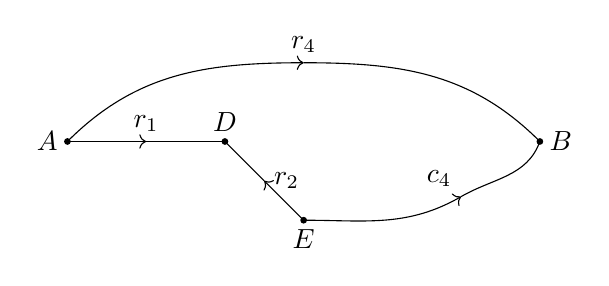
\begin{tikzpicture}
    \filldraw[black](0,0)circle(1pt);
    \filldraw[black](2,0)circle(1pt);
    %\filldraw[black](4,0)circle(1pt);
    \filldraw[black](6,0)circle(1pt);
    \filldraw[black](3,-1)circle(1pt);

    \draw[->](0,0)to[out=45,in=180](3,1)node[above]{$r_4$};
    \draw[-](3,1)to[out=0,in=135](6,0);

    \draw[->](0,0)node[left]{$A$}--(1,0)node[above]{$r_1$};
    \draw[-](1,0)--(2,0)node[above]{$D$};

    %\draw[->](2,0)--(3,0)node[above]{$4$};
    %\draw[-](3,0)--(4,0);

    %\draw[->](4,0)node[above]{$C$}--(5,0)node[above]{$r_3$};
    %\draw[-](5,0)--(6,0);

    %\draw[->](3,-1)to[out=180,in=330](1,-0.7)node[above right]{$1$};
    %\draw[-](1,-0.7)to[out=150,in=290](0,0);

    \draw[->](3,-1)node[below]{$E$}--(2.5,-0.5)node[right]{$r_2$};
    \draw[-](2.5,-0.5)--(2,0);

    %\draw[-](3,-1)--(3.5,-0.5)node[right]{$5$};
    %\draw[->](4,0)--(3.5,-0.5);

    \draw[->](3,-1)to[out=0,in=210](5,-0.7)node[above left]{$c_4$};
    \draw[-](5,-0.7)to[out=30,in=250](6,0)node[right]{$B$};
\end{tikzpicture}
\end{document}